\documentclass{article}

% Formatting
\DeclareUnicodeCharacter{2060}{\nolinebreak} % Prevent unicode (U+2060) error on local complile
\frenchspacing % No double spacing between sentences
\hbadness=1000000 % Turn off \hbox badness warnings
\linespread{1.2} % Set linespace

% Packages
\usepackage[a4paper, left=1.5cm, right=1.5cm, top=2.0cm, bottom=2.0cm]{geometry}
\usepackage{authblk} % For author formatting
\usepackage{caption} % For figure and table captions
\usepackage{cclicenses} % For creative commons license
\usepackage{float} % To force figure location after text
\usepackage{graphicx} % Adds more functionality to graphics for inclusion of figures
%\usepackage{hyperref} % For clickable web links
\usepackage{lscape} % For landscape pages
\usepackage{lineno} % Allows use of \linenumbers to add line numbers 
\usepackage{lmodern} % A scalable font - avoids erros due to non-sclabale fonts
\usepackage{longtable,booktabs}  % For tables
\usepackage{makecell} % For cell formatting in tables
\usepackage{markdown} % allow use of markdown syntax
\usepackage{microtype} % 'Improved' typesetting
\usepackage[nottoc, numbib]{tocbibind} % Add references to table of contents, and make it a numbered section
\usepackage{parskip} % Adds white space between paragraphs
\usepackage{pdflscape} % To create landscape pages that show as landscape in PDF viewer
\usepackage{ragged2e} % Better right ragged edges (allows hyphenation)
\usepackage{subcaption} % Allows use of subfigures
\usepackage[super]{natbib} % Citations using superscript
\usepackage{titlesec} % For title spacing
\usepackage[toc,page]{appendix}
\usepackage{url} % Tidy web links
\usepackage[utf8]{inputenc}
\usepackage{verbatim}
\usepackage{xcolor} % For coloured text
\usepackage{xurl} % For url but with more flexible linebreaking
\usepackage{placeins} % to use \FloatBarrier where want a hard break between content (to force and order of text and figures
\usepackage[hidelinks]{hyperref}




% Info on wordcounts:
% https://www.overleaf.com/learn/how-to/Is_there_a_way_to_run_a_word_count_that_doesn%27t_include_LaTeX_commands%3F

% To include refs in word count:
%TC:incbib

\newcommand{\detailtexcount}[1]{%
  \immediate\write18{texcount -merge -sum -q #1.tex output.bbl > #1.wcdetail }%
  \verbatiminput{#1.wcdetail}%
}

% Count tables in wordcount (change to 0 0 if tables not included in word count)
%TC:group table 0 1
%TC:group tabular 1 

\begin{document}


% Ignore title and abstract in word count
%TC:ignore
\title{\textbf{Modelling thrombectomy provision in England, 2026}\\[0.5em]
       \large \textbf{The effect of addition thrombectomy provision in Taunton and Worcester}}

\author[1,2]{Michael Allen}
\author[1,2]{Anna Laws}
\author[1,2]{Yinghui Wei}
\author[1,2]{Martin James}
% Check affiliations - update RDE Name
\affil[1]{\footnotesize University of Exeter Medical School}
\affil[2]{\footnotesize NIHR Applied Research Collaboration South West}


%\date{}
\begin{figure}
    \centering
    
\includegraphics[height=1.6cm]{images/arc_logo.png}
    \hspace{3em}%
    
\includegraphics[height=1.85cm]{images/university-of-exeter-logo.png}
\end{figure}


\maketitle

% Table of contents


\tableofcontents



\section{Introduction}

Stroke is a leading cause of death and of adult disability in the United Kingdom, with more than 100,000 strokes each year. Around 85\% are ischaemic, caused by occlusion of a cerebral artery. Two emergency treatments aim to restore blood flow to the affected brain before the damage becomes permanent: intravenous thrombolysis (IVT), in which a clot-dissolving drug is given by infusion, and mechanical thrombectomy (MT), in which the clot is physically removed through a catheter. The benefit of both depends heavily on how quickly they are delivered.

\subsection{Intravenous thrombolysis}

IVT with alteplase was established by randomised trials showing benefit when given within 3 hours of onset \cite{ninds1995}, later extended to 4.5 hours \cite{hacke2008}. The individual patient data meta-analysis of Emberson et al., pooling 6{,}756 patients from nine trials, quantified how strongly that benefit depends on time \cite{emberson_effect_2014}. The odds of an excellent outcome (modified Rankin Scale, mRS, 0--1 at 3--6 months) were increased by 75\% when treatment was given within 3 hours (OR 1.75, 95\% CI 1.35--2.27) and by 26\% between 3 and 4.5 hours (OR 1.26, 95\% CI 1.05--1.51), with no significant benefit beyond 4.5 hours (OR 1.15, 95\% CI 0.95--1.40). In absolute terms this is roughly ten additional patients per 100 treated achieving an excellent outcome if treated within 3 hours, falling to about five per 100 between 3 and 4.5 hours. Alteplase increased the risk of fatal intracranial haemorrhage in the first week by about 2 percentage points, a risk that did not diminish with later treatment, so the balance of benefit and harm worsens as time passes. IVT can be delivered at any acute stroke unit with access to brain imaging, but it is relatively ineffective at recanalising large, proximal clots.

\subsection{Mechanical thrombectomy}

MT is suitable for patients with large vessel occlusion (LVO) of the anterior circulation, who account for a minority of ischaemic strokes but a disproportionate share of death and severe disability. The HERMES collaboration pooled individual data on 1{,}287 patients from five trials and found that MT substantially reduced disability at 90 days (OR 2.49, 95\% CI 1.76--3.53), with functional independence (mRS 0--2) in 46.0\% of treated patients against 26.5\% of controls, and a number needed to treat of 2.6 for one patient to improve by at least one mRS level \cite{goyal2016}. This makes MT one of the most effective interventions in acute medicine.

As with IVT, the effect diminishes with delay. In the MR CLEAN trial, Fransen et al.\ found that the absolute benefit of MT on functional independence fell by about 6 percentage points for every hour of delay to reperfusion, from an estimated 25.9\% with reperfusion at 3 hours to 6.7\% at 6 hours \cite{fransen_time_2016}. The HERMES time-to-treatment meta-analysis confirmed the pattern across trials: each hour of delay to reperfusion was associated with worse disability (common OR 0.84, 95\% CI 0.76--0.93), and the benefit of MT over IVTas no longer statistically significant beyond 7.3 hours from onset \cite{saver2016}. Later trials showed that patients selected by advanced imaging can still benefit up to 24 hours after they were last known to be well \cite{nogueira2018,albers2018}, but these patients are a selected subgroup, and earlier treatment remains better for them too.

\subsection{The importance of time}

The time dependence of both treatments reflects the underlying biology. In a typical untreated large vessel stroke an estimated 1.9 million neurons are lost each minute \cite{saver2006}. Translated into patient outcomes, each minute saved in delivering IVT has been estimated to give 1.8 extra days of healthy life \cite{meretoja2014}, and each minute saved in delivering MT gives  an extra 4.2 days \cite{meretoja2017}. Time to treatment is therefore a primary determinant of outcome rather than just a secondary operational concern.

\subsection{Implications for the organisation of services}

The two treatments place different demands on a health system. IVT is widely available, whereas MT requires neurointerventional expertise and facilities and is concentrated in a small number of specialist centres; in England it has been provided by 24 neuroscience centres. Patients who live far from one of these centres either travel further to reach it directly, delaying IVT, or attend a local IVT-only unit first for earlier IVT, and are then transferred, delaying MT. Around 10\% of patients admitted with stroke are estimated to be eligible for MT \cite{mcmeekin2017}, and the NHS Long Term Plan set the ambition of reaching this level \cite{nhsltp2019}. In 2024/25, however, 4.4\% of stroke patients received MT and 12.2\% received IVT \cite{ssnap2025}.

\subsection{The addition of two new MT units}

Because the benefit of MT decays so quickly, the number and location of MT units directly affect both how many patients can be treated and how much each of them gains \cite{allen2019}. This report examines the expected effect of adding two new MT units in England, at Taunton and Worcester. In order to isolate the effect of geography, it is assumed all stroke units perform similarly.
\section{Methods}

Full methods have been published \cite{laws2025modelling}.

\subsection{Lower Super Output Areas (LSOA)}

We performed our analysis across England using LSOA as our geographic footprint \cite{ons}. LSOAs are small areas in England, with roughly 1,500 people in each area. There are 32,843 LSOAs in England.

\subsection{Travel times}

Travel times between all Lower Super Output Areas (LSOAs, areas with a population of approximately 1,500) and all stroke units were estimated using Open Street Map data \footnote{\url{https://www.openstreetmap.org/}} and the Routino \footnote{\url{https://www.routino.org/}} route finding engine on Linux.

\subsection{Outcome modelling}

Outcome modelling is based on published meta-analysis of clinical trials which have evaluated the decline of effectiveness  of IVT and MT over time \cite{emberson_effect_2014, fransen_time_2016}. We have applied those models to the expected real world treatment population (based on the national stroke audit of England and Wales, SSNAP). We calculated the expected benefit in the treated population for non large vessel occlusion (\textit{nLVO}, receiving IVT only) and large vessel occlusion (\textit{LVO}, receiving IVT and/or MT) separately.

We used modified Rankin Scale (mRS) at 3--6 months as a measure of outcome. mRS is the most commonly used instrument to describe post-stroke functional outcome \cite{quinn_functional_2009}, describing independence of living from a scale of 0 (no disability) through to 5 (severe disability requiring constant nursing attention), with death assigned an mRS of 6. A commonly used surrogate for independent living is mRS 0--2.

We calculated the patients' mRS outcome distribution based on time to treatment for three patient-treatment cohorts: nLVO treated with IVT; LVO treated with IVT alone; and LVO treated with IVT and MT. For each patient-treatment cohort we calculated an mRS distribution for treatment at any given time by interpolating between the mRS distribution for treatment given at \emph{t=0} (time of stroke onset) and the mRS distribution for treatment given at \emph{t=No Effect} (time of no effect of treatment), assuming that log odds of achieving any given mRS threshold fall linearly over time \cite{emberson_effect_2014, fransen_time_2016}. As possible changes to service provision reported here should only affect potential candidates for thrombectomy, in this report we only show results for treated large vessel occlusion stroke.

The time to no effect was 6.3 hours for IVT \cite{emberson_effect_2014} and 8.0 hours for MT \cite{ fransen_time_2016}. Our model did not include selection of patients who may still benefit from treatment beyond these durations through the use of perfusion scanning. This number is small for IVT, but is more substantial for MT – approximately 2500 per annum in England.

Our modelling compares outcomes for those patients receiving IVT and MT. We do not make any assumption about the proportion of all patients receiving those treatments.

Code for outcome modelling, and a further description of methods is available on GitHub \footnote{\url{https://github.com/stroke-modelling/stroke-outcome/}}, and we have made it available as a Python package on PyPi \footnote{\url{https://pypi.org/project/stroke-outcome/}}. We have described the methods in detail in an online book \footnote{\url{https://samuel-book.github.io/stroke_outcome/intro.html}}.

\subsection{Process times}

To study geographic variation in benefit of MSU care, a single set of parameters was chosen that reflected a reasonable base case for performance of usual care of LVO stroke. Process times (minutes) are shown in the following list.

\vspace{5mm}

\begin{minipage}{1.0\textwidth}  % Define the width of the minipage
\begin{itemize}
    \item Stroke onset to call: 30
    \item Call to ambulance arrival: 20
    \item Ambulance on-scene: 30
    \item Travel time to first admitting unit: Depends on geography
    \item Hospital arrival to IVT: 30
    \item If transfer for MT required:
    \begin{itemize}
        \item Transfer-related net MT delay (excluding travel time)*: 60
        \item Transport time to MT unit: Depends on geography
    \end{itemize}
    \item Hospital arrival to MT: 90
\end{itemize}

*This assumes a typical door-in-door-out time of 90 mints at the IVT-only centre, but 1 30 minute reduction in Hospital arrival to MT at the transferred-in MT centre, due to work already performed at the IVT-only unit.
\end{minipage}



\section{Results}

\subsection{2025 thrombectomy performance statistics (from SSNAP)}

In 2025, 4.8\% of all emergency stroke admissions received MT. The use for ischaemic stroke was 5.6\%. The use for ischaemic stroke with a stroke severity (NIHSS) of 11+ was 22.1\%.

For ischaemic strokes with NIHSS 11+, the MT rate depending on the type of first admitting unit was:

\begin{itemize}
    \item First admitted to MT unit (do not require transfer for MT) = 24.7\%
    \item First admitted to IVT-only unit (require transfer for MT) = 16.5\%
    \item \textit{Summary}: MT rate for patients requiring transfer is 67\% of those not requiring transfer
\end{itemize}

The above analysis has informed our modelling: for scenarios including onward transfers for MT from IVT-only units, we have also modelled the effect of a 33\% MT loss for those transferred from an IVT-only unit.

The first arrival to thrombectomy times (median and quartiles) were:

\begin{itemize}
    \item First admitted to MT unit = 128 mins (95-183 mins)
    \item First admitted to IVT-only unit = 241 mins (182-308 mins)
    \item \textit{Summary}: 113 mins delayed MT (on average) when transfer required (includes transfer-related net delay and transport time)
\end{itemize}

\subsection{Clinical benefit of reperfusion treatment (modelled results)}

\subsubsection{Clinical benefit of current system}

In the current system (including new MT units in East Kent and Norwich), without reperfusion treatment the model predicts 26.5\% of LVO patients would achieve a good outcome (mRS 0-2 at 3-6 months). With IVT alone, this would increase to 32.4\% for treated LVO patients, and with IVT and MT there would be a further increase to 37.8\%. If all LVO patients attended their closest MT unit first (a \textit{mothership} model of care) 42.0\% of treated LVO patients would achieve a good outcome (mRS 0-2 at 3-6 months). Directing as many treatable LVO patients to their closest MT unit would maximise outcomes.

There is significant variation in clinical benefit by geography, even without loss of MT procedures for patients who first attend an IVT-only unit. Total travel time to an MT unit, including transfer time when required, ranges from 0 to 192 minutes (including a net non-travel time delay to MT of 60 minutes for transfer). The proportion of treated patients who achieve a good outcome (mRS 0-2 at 3-6 months) ranges from 31.8\% to 39.8\% in England (a benefit of treatment of between 5.4 and 13.3 percentage points increase in a good outcome, mRS 0-2 at 3-6 months). Those living closest to an MT unit have the greatest benefit from treatment, with the least benefit for those with the longest time to MT (a combination of travel time to their closest IVT-only unit, non-travel transfer-related delays, and the travel time from that IVT unit to the closest MT unit).

\subsubsection{Clinical benefit of planned system (2 additional MT units)}

We have compared the expected benefit of the current system (including new MT units in East Kent and Norwich) to the same system with the addition of MT units at Taunton and Worcester.

The addition of a new MT unit in Taunton potentially benefits a catchment population of 2,736 stroke admissions per year. The net improvement is expected to be about 2.9 additional good outcomes (mRS 0-2 at 3-6 months) if there is no loss of MT for patients first admitted to an IVT-only unit.

The addition of a new MT unit in Worcester potentially benefits a catchment population of 2,010 stroke admissions per year. The net improvement is expected to be about 2.7 additional good outcomes (mRS 0-2 at 3-6 months) if there is no loss of MT for patients first admitted to an IVT-only unit.

Improvement in outcomes is not even across the population who may benefit. The benefit is greatest for those who attend the new MT unit directly, as they benefit most in receiving earlier MT, and do not risk the lower MT rates for patients first attending an IVT-only unit. The benefit for patients currently attending Taunton or Worcester is an increase of 7.1 and 5.5 percentage points in treated LVO with a good outcome (mRS 0-2 at 3-6 months), if there is no loss of MT by first attending an IVT-only unit. This improvement rises to 8.1 and 7.1 percentage points if there is a 33\% loss in MT first attending an IVT-only unit (as these patients avoid a loss in MT due to transfer). The benefit to patients first attending an IVT-only unit ranges from 0.05 to 1.5 percentage points with no loss of MT, or 0.04 to 0.96 percentage points with a 33\% loss in MT. The benefit to patients first attending Dorchester is extremely marginal (approx 0.05 increase in percentage points) as travel times to Taunton and Southampton are very similar (and which unit is the shortest travel time may vary during, and between, days). More details are given in table \ref{tab:ivt-location}.

\begin{table}[H]
  \centering
  \caption{Clinical benefit for treated LVO patients (percentage points increase with a good outcome, mRS 0-2 at 3-6 months, for 100 patients treated) due to the addition of Taunton and Worcester as MT units. Results shown by first-attending unit, including with, and without, a 33\% loss of MT for patients first attending an IVT-only unit.} 
  \label{tab:ivt-location}
  \begin{tabular}{lrr}
    \toprule
    IVT location & No MT loss & 33\% MT loss \\
    \midrule
    Taunton     & 7.13 & 8.11 \\
    Worcester   & 5.55 & 7.13 \\
    Hereford    & 1.51 & 1.01 \\
    Barnstaple  & 1.43 & 0.96 \\
    Exeter      & 1.04 & 0.69 \\
    Cheltenham  & 0.92 & 0.62 \\
    Dorchester  & 0.05 & 0.04 \\
    \bottomrule
  \end{tabular}
\end{table}

\subsubsection{Maps of travel times and clinical benefit}

Figures \ref{fig:map_current_no_loss} to \ref{fig:map_new_lossy} show maps of the current (figures \ref{fig:map_current_no_loss}, \ref{fig:map_current_lossy}) and planned system (with additional MT units at Taunton and Worcester) (figures \ref{fig:map_new_no_loss} and \ref{fig:map_new_lossy}), with and without a 33\% loss of MT for patients first attending an IVT-only unit. Figures \ref{fig:comparison_three_in_one} and \ref{fig:comparison_three_in_one_lossy} map the impact of adding two MT units on the travel time and clinical benefit for the affected areas.

% Base case
\begin{figure}[H]
\centering
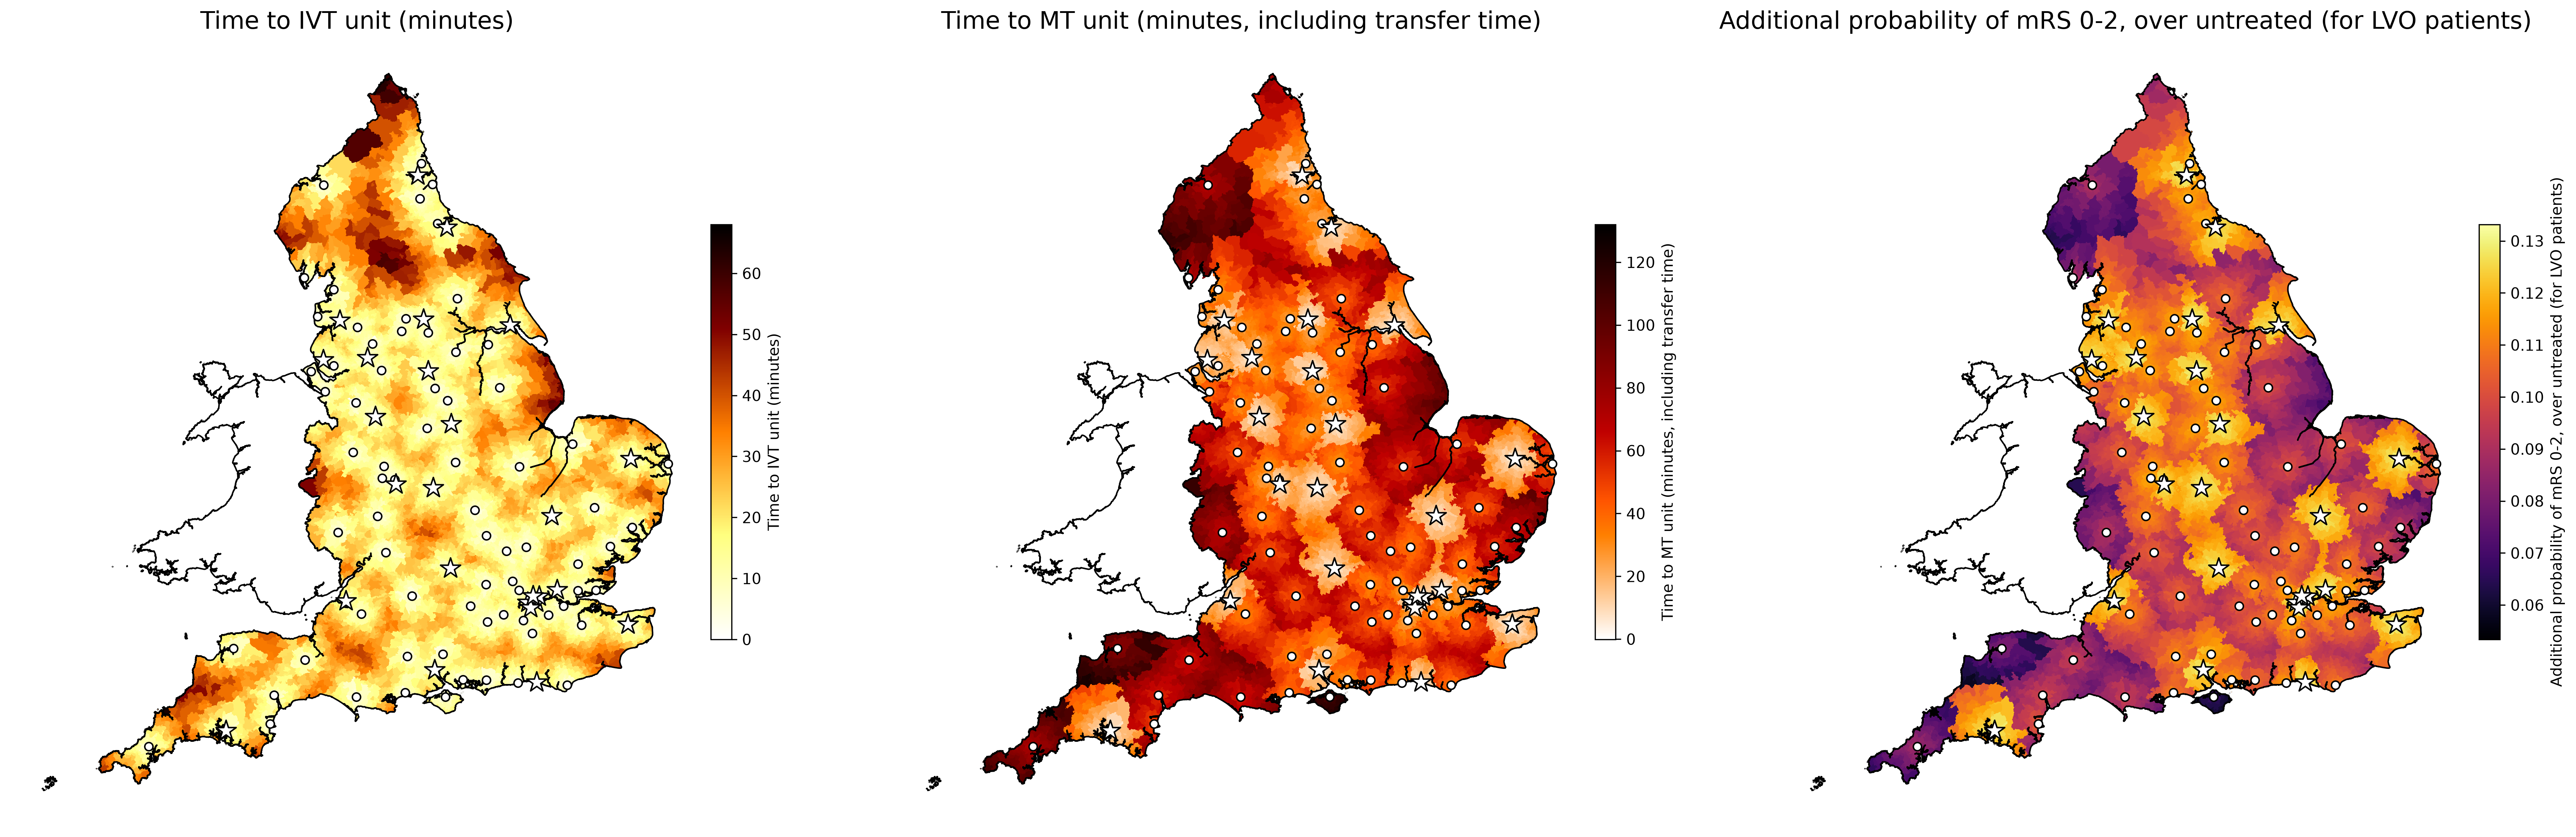
\includegraphics[width=\linewidth]{images/map_three_in_one_current_hospitals_lvo.png} 
\caption{Modelled times and outcomes for stroke patients with large vessel occlusion receiving thrombolysis (IVT) and thrombectomy (MT), with current IVT/MT provision (Taunton and Worcester as IVT-only units) and no loss of MT by first attending an IVT-only unit. \textit{Left}: Predicted travel times to closest (in time) IVT unit. \textit{Middle}: Total travel time to MT unit; this includes travel time to closest IVT unit, a net delay before transfer of 60 minutes, and travel time from IVT unit to MT unit. \textit{Right}: The predicted improvement in the proportion of treated LVO patients with mRS 0-2 at 3-6 months, assuming there is no loss of use of MT by first attending an IVT-only unit. Stroke teams are shown as stars (providing both IVT and MT) or circles (providing IVT alone).}
\label{fig:map_current_no_loss}
\end{figure}

% Base case - loss pf MT
\begin{figure}[H]
\centering
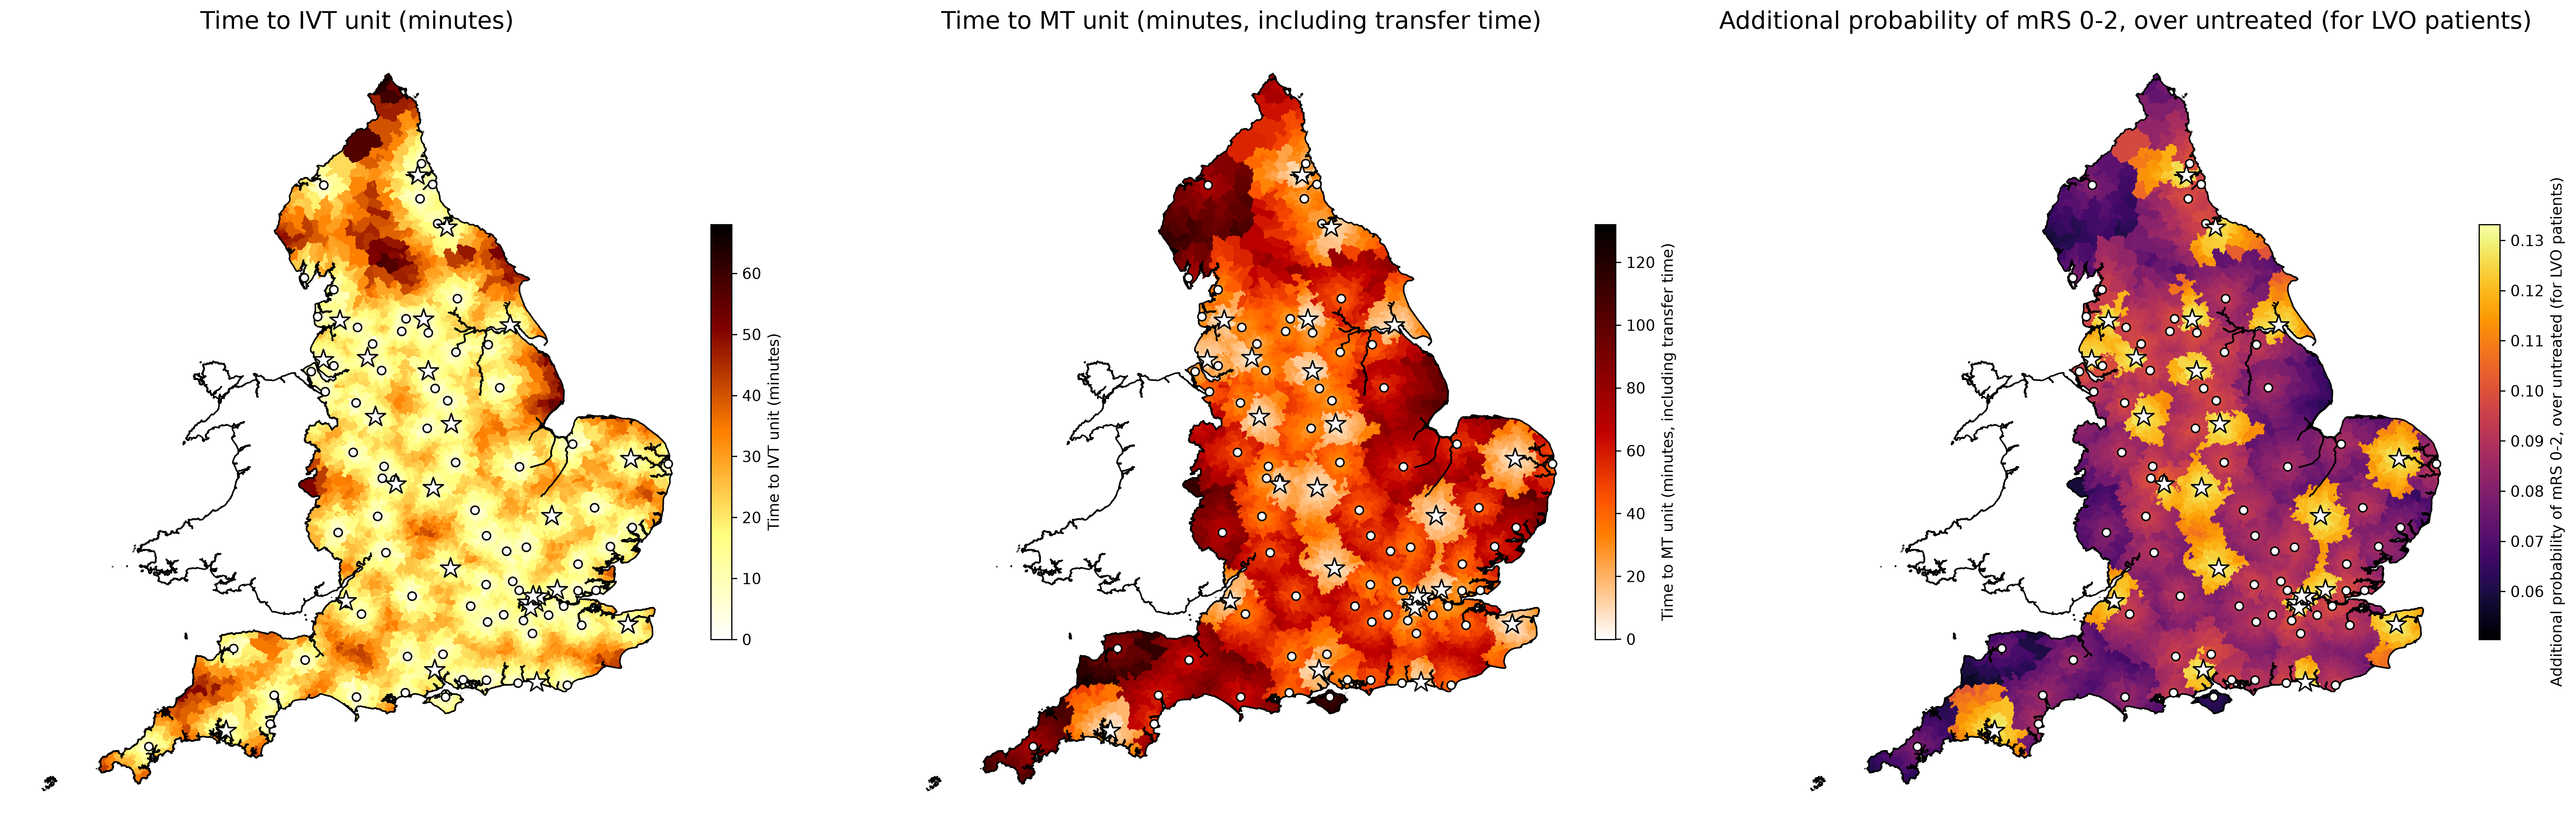
\includegraphics[width=\linewidth]{images/map_three_in_one_current_hospitals_67_percent_transfer_lvo.png} 
\caption{Modelled times and outcomes for stroke patients with large vessel occlusion receiving thrombolysis (IVT) and thrombectomy (MT), with current IVT/MT provision (Taunton and Worcester as IVT-only units) and 33\% loss of use of MT by first attending an IVT-only unit. \textit{Left}: Predicted travel times to closest (in time) IVT unit. \textit{Middle}: Total travel time to MT unit; this includes travel time to closest IVT unit, a net delay before transfer of 60 minutes, and travel time from IVT unit to MT unit. \textit{Right}: The predicted improvement in the proportion of treated LVO patients with mRS 0-2 at 3-6 months, assuming a 33\% loss of use of MT by first attending an IVT-only unit. Stroke teams are shown as stars (providing both IVT and MT) or circles (providing IVT alone).}
\label{fig:map_current_lossy}
\end{figure}


  
% Worcester + Taunton
\begin{figure}[H]
\centering
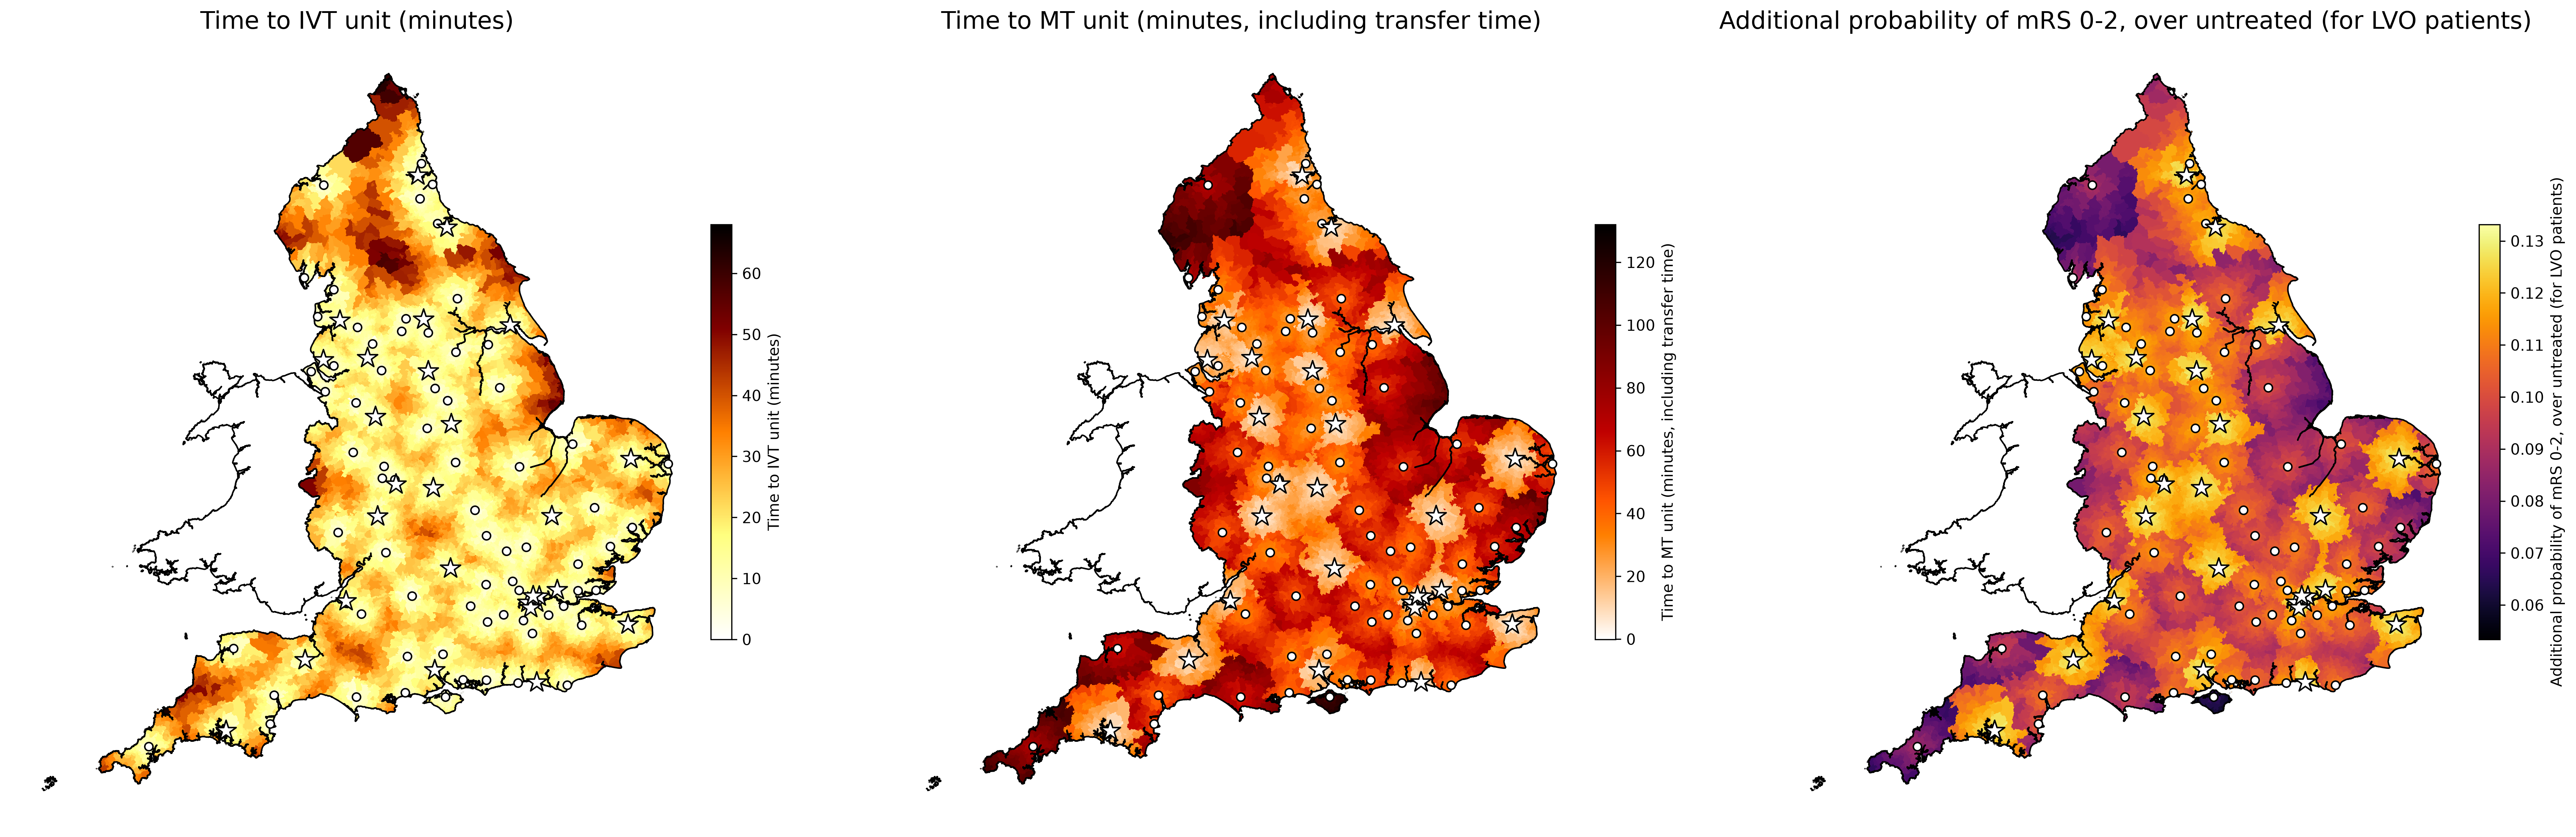
\includegraphics[width=\linewidth]{images/map_three_in_one_taunton_and_worcester_lvo.png}  
\caption{Modelled times and outcomes for stroke patients with large vessel occlusion receiving thrombolysis (IVT) and thrombectomy (MT), with the addition of Taunton and Worcester providing MT, no loss of MT by first attending an IVT-only unit, and with the addition of Taunton and Worcester providing MT. \textit{Left}: Predicted travel times to closest (in time) IVT unit. \textit{Middle}: Total travel time to MT unit; this includes travel time to closest IVT unit, a net delay before transfer of 60 minutes, and travel time from IVT unit to MT unit. \textit{Right}: The predicted improvement in the proportion of treated LVO patients with mRS 0-2 at 3-6 months, assuming there is no loss of use of MT by first attending an IVT-only unit. Stroke teams are shown as stars (providing both IVT and MT) or circles (providing IVT alone).}
\label{fig:map_new_no_loss}
\end{figure}

% Worcester + Taunton - loss pf MT
\begin{figure}[H]
\centering
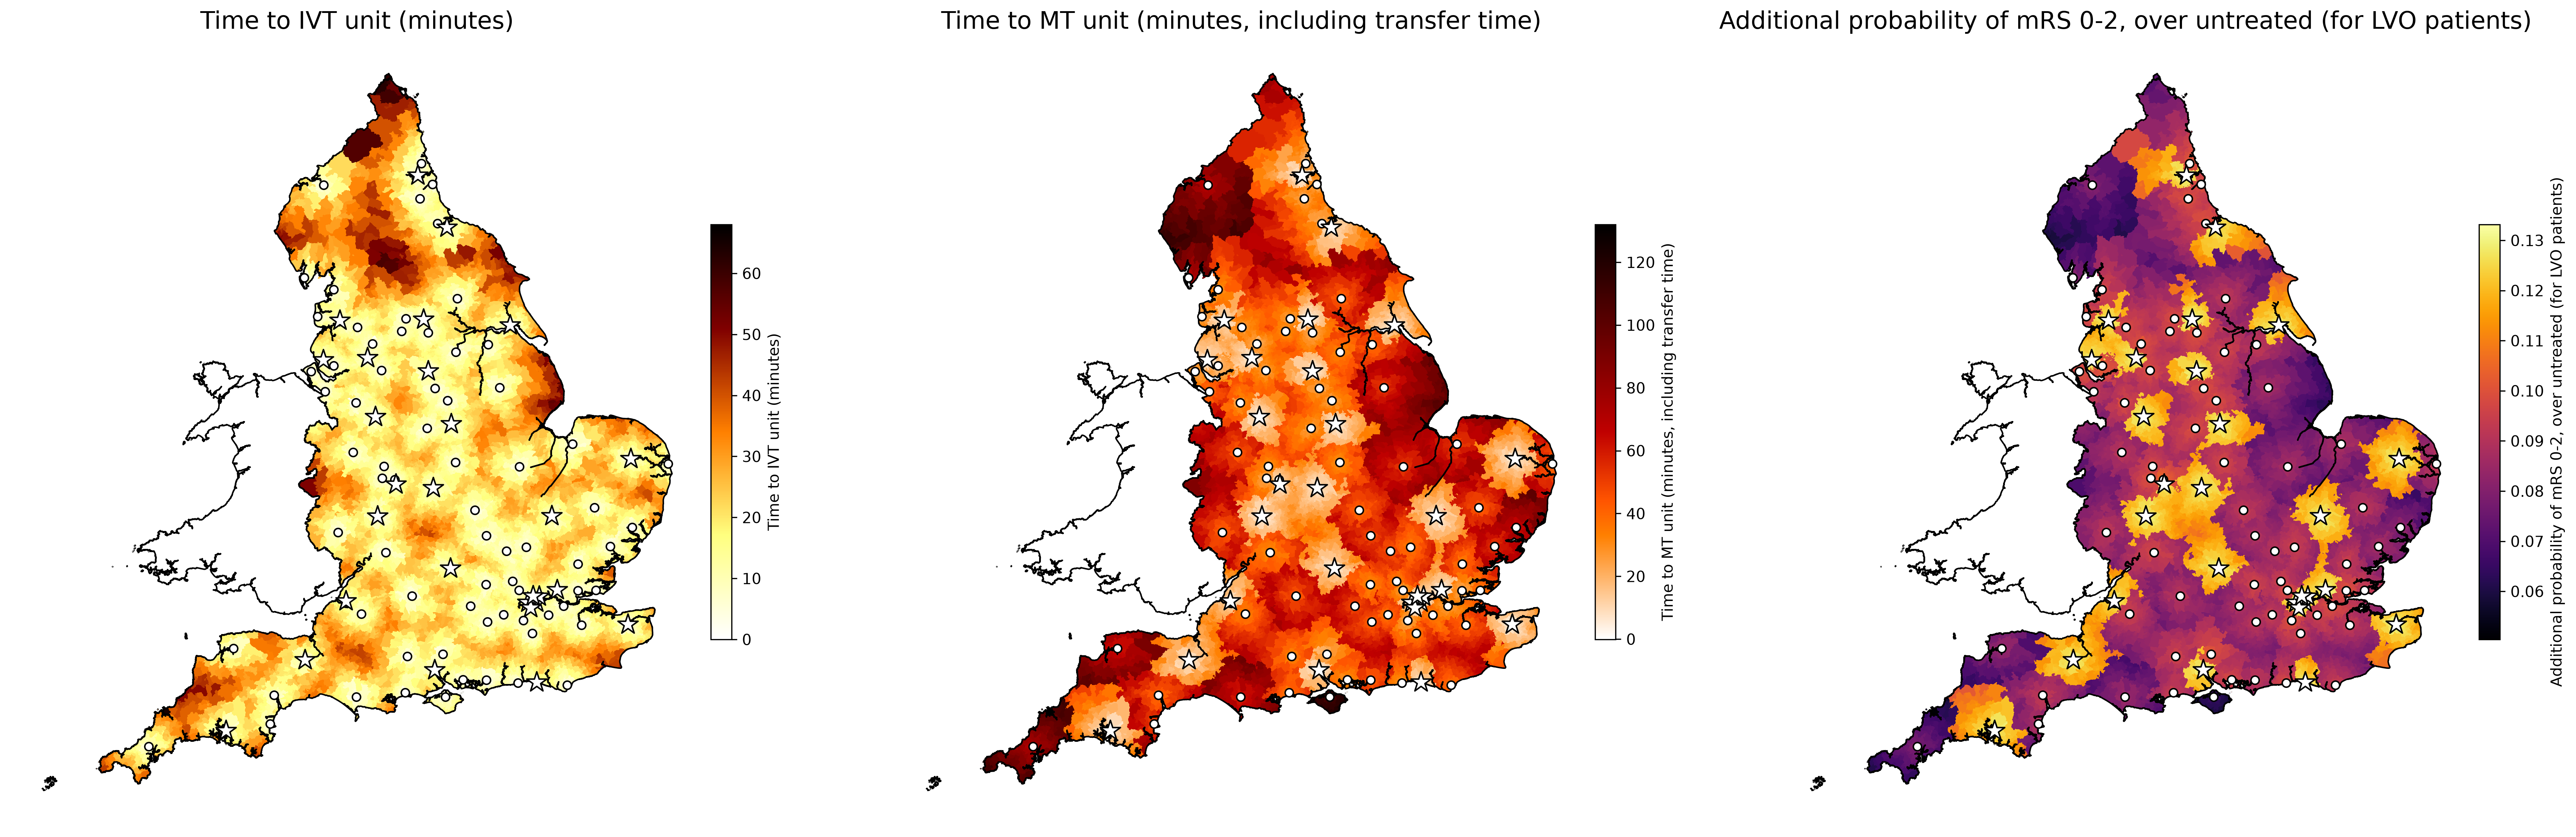
\includegraphics[width=\linewidth]{images/map_three_in_one_taunton_and_worcester_67_percent_transfer_lvo.png} 
\caption{Modelled times and outcomes for stroke patients with large vessel occlusion receiving thrombolysis (IVT) and thrombectomy (MT), with the addition of Taunton and Worcester providing MT, 33\% loss of use of MT by first attending an IVT-only unit, and with the addition of Taunton and Worcester providing MT. . \textit{Left}: Predicted travel times to closest (in time) IVT unit. \textit{Middle}: Total travel time to MT unit; this includes travel time to closest IVT unit, a net delay before transfer of 60 minutes, and travel time from IVT unit to MT unit. \textit{Right}:  The predicted improvement in the proportion of treated LVO patients with mRS 0-2 at 3-6 months, assuming a 33\% loss of use of MT by first attending an IVT-only unit. Stroke teams are shown as stars (providing both IVT and MT) or circles (providing IVT alone).}
\label{fig:map_new_lossy}
\end{figure}


% Comparison maps


\begin{figure}[H]
    \centering
    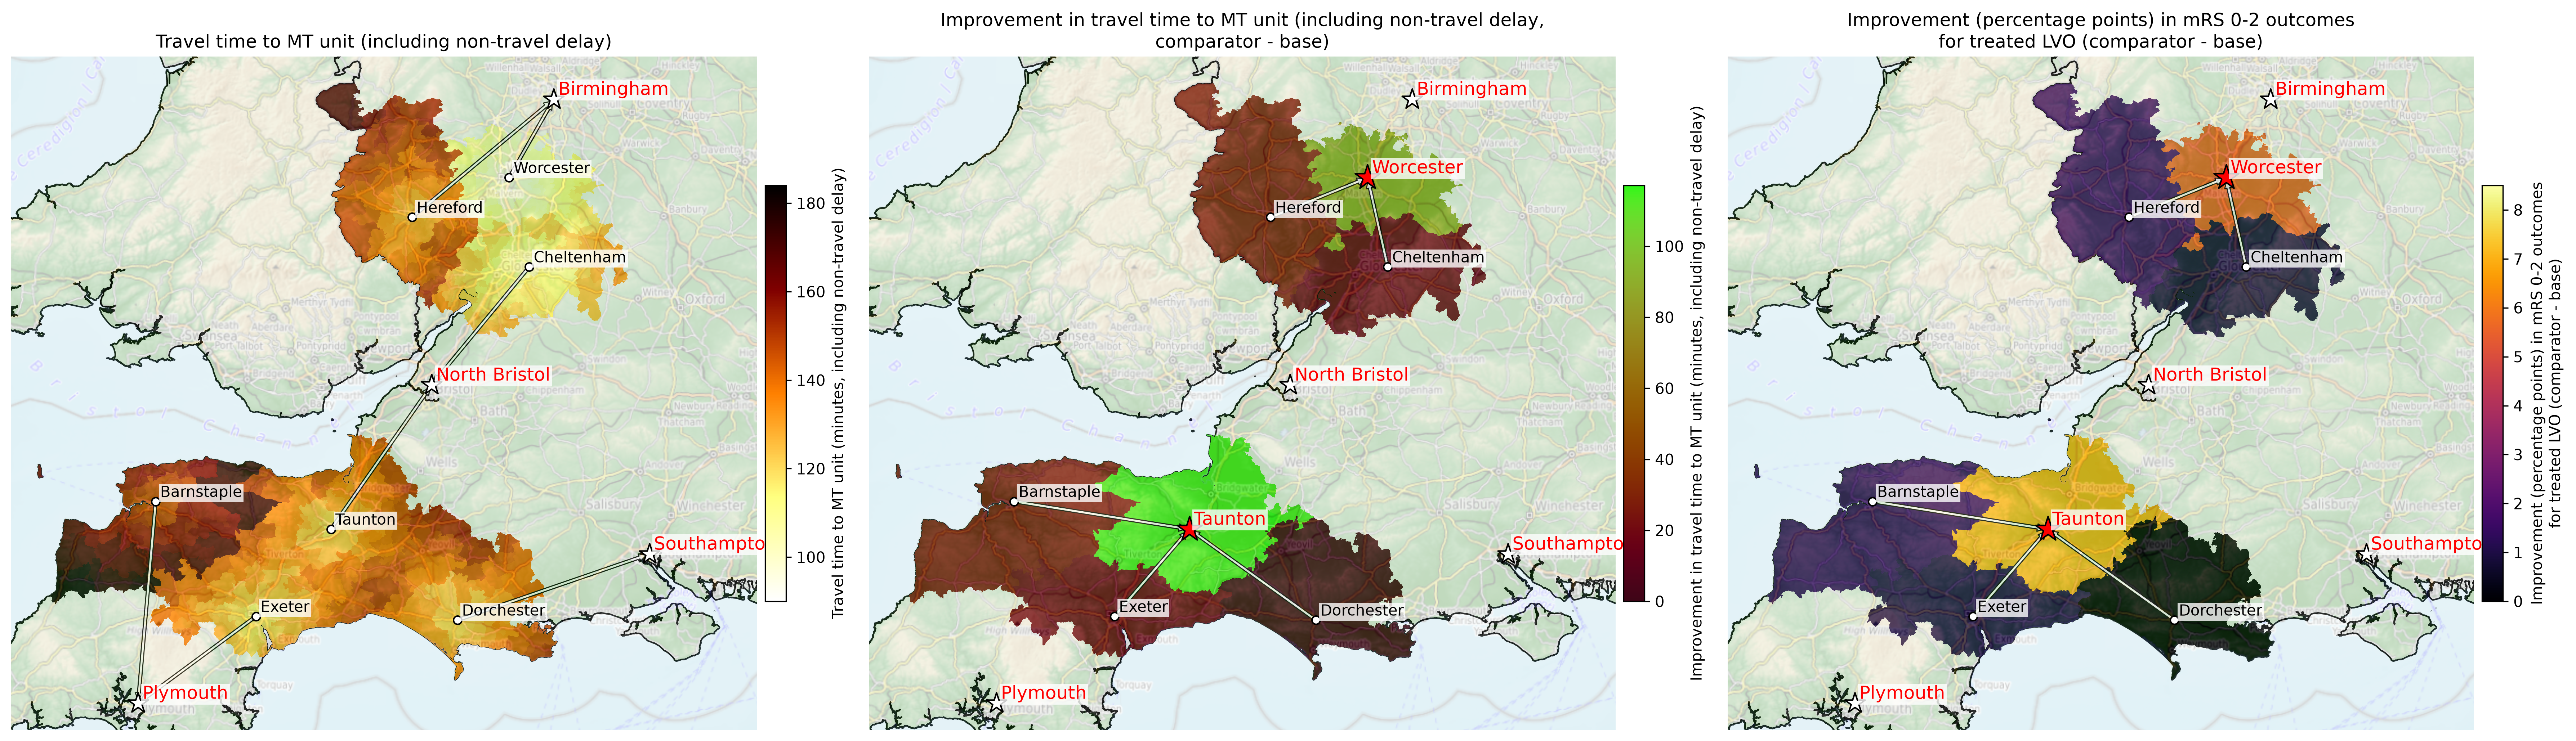
\includegraphics[width=1\linewidth]{images/comparison_map_three_in_one_taunton_worcester.png}
    \caption{Comparison of travel times for MT (including non-travel delays) and outcomes (the predicted improvement in the proportion of treated LVO patients with mRS 0-2 at 3-6 months) by adding MT capability at Taunton and Worcester, with no loss of MT by first attending an IVT-only unit. The arrows indicate the modelled transfer destination from IVT-only units. \textit{Left}: Current predicted travel times for MT, \textit{Middle}: Improvement in travel time to MT. \textit{Right}: Improvement in outcomes.}
    \label{fig:comparison_three_in_one}
\end{figure}

\begin{figure}[H]
    \centering
    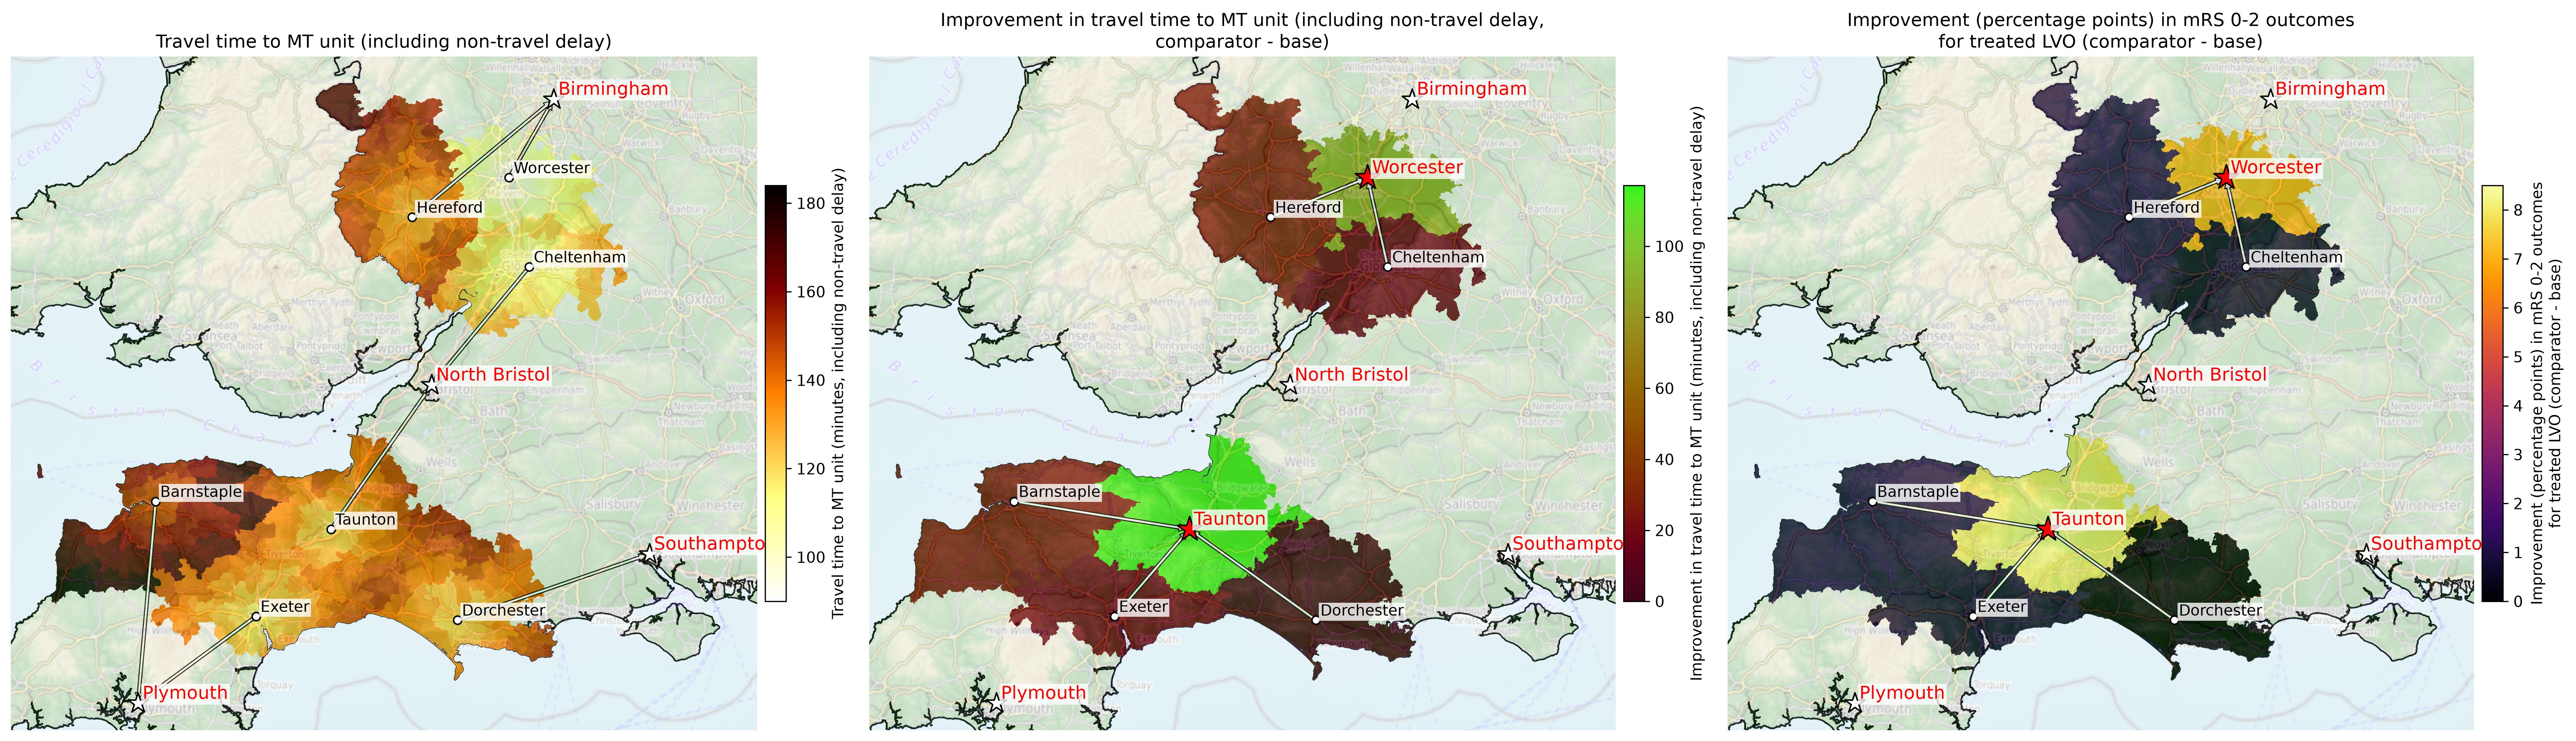
\includegraphics[width=1\linewidth]{images/comparison_map_three_in_one_taunton_worcester_67_percent_transfer.png}
    \caption{Comparison of travel times for MT (including non-travel delays) and outcomes (the predicted improvement in the proportion of treated LVO patients with mRS 0-2 at 3-6 months) by adding MT capability at Taunton and Worcester, with 33\% loss of MT by first attending an IVT-only unit. The arrows indicate the modelled transfer destination from IVT-only units. \textit{Left}: Current predicted travel times for MT, \textit{Middle}: Improvement in travel time to MT. \textit{Right}: Improvement in outcomes.}
    \label{fig:comparison_three_in_one_lossy}
\end{figure}



\subsection{MT admissions of planned system (2 additional MT units)}

Table \ref{tab:mt_units} shows the effect of adding MT units at Taunton and Worcester on MT admissions at MT units in the affected region, if there was no loss of chance to receive MT by first attending an IVT-only unit.

\begin{table}[htbp]
\centering
\caption{Current and planned mechanical thrombectomy (MT) activity by MT unit, including additional MT units at Taunton and Worcester.}
\label{tab:mt_units}
\begin{tabular}{l|c|c|c}
\hline
\textbf{MT Unit} & \textbf{Current MT*} & \textbf{Planned MT*} & \textbf{Change} \\
\hline
Birmingham    & 707 & 585 & $-122$ \\
North Bristol & 393 & 219 & $-174$ \\
Plymouth      & 341 & 231 & $-110$ \\
Southampton**   & 558 & 488 & $-70$  \\
Taunton**     & 0   & 273 & 273    \\
Worcester     & 0   & 202 & 202    \\
\hline
\end{tabular}

\vspace{1.0em}
\begin{minipage}{0.85\linewidth}
\small
*The destination MT unit is chosen as the closest available unit to the first admitting IVT unit. Numbers assume 10\% of all stroke receive MT, with no loss by transfer.\\
**About 70 of Taunton’s MT come from Dorchester (where benefit is negligible compared with current use of Southampton for MT).
\end{minipage}
\end{table}

\subsection{Introducing a travel bias towards selecting an MT unit}

Figures \ref{fig:map_current_bias} and \ref{fig:map_taunton_worcester_bias} show maps of travel times and outcomes for treated LVO patients if patients are taken directly to an MT unit if travel time is no longer than 10 minutes more than first attending a closer IVT-only unit.

For the current provision of MT, a summary of key results is:

\begin{itemize}
    \item Without travel bias, mean percentage point increase in treated LVO with good outcome (mRS 0-2 at 3-6 months) = 12.6 (11.6 with 33\% transfer loss of MT). 33\% admission are direct to MT unit.
    \item With 10 minute travel bias, percentage point increase in treated LVO with good outcome (mRS 0-2 at 3-6 months) = 14.0  (13.4 with 33\% transfer loss of MT). 55\% admission are direct to MT unit.
    \item With 15 minute travel bias, percentage point increase in treated LVO with good outcome (mRS 0-2 at 3-6 months) = 14.8 (14.4 with 33\% transfer loss of MT). 67\% admission are direct to MT unit.
\end{itemize}

With the addition of Taunton and Worcester as MT units, a summary of key results is:

\begin{itemize}
    \item Without travel bias, mean percentage point increase in treated LVO with good outcome (mRS 0-2 at 3-6 months) = 12.7 (11.8 with 33\% transfer loss of MT). 35\% admission are direct to MT unit.
    \item With 10 minute travel bias, percentage point increase in treated LVO with good outcome (mRS 0-2 at 3-6 months) = 14.2  (13.6 with 33\% transfer loss of MT). 57\% admission are direct to MT unit.
    \item With 15 minute travel bias, percentage point increase in treated LVO with good outcome (mRS 0-2 at 3-6 months) = 15.0 (14.6 with 33\% transfer loss of MT). 69\% admission are direct to MT unit.
\end{itemize}

\begin{figure}[H]
    \centering
    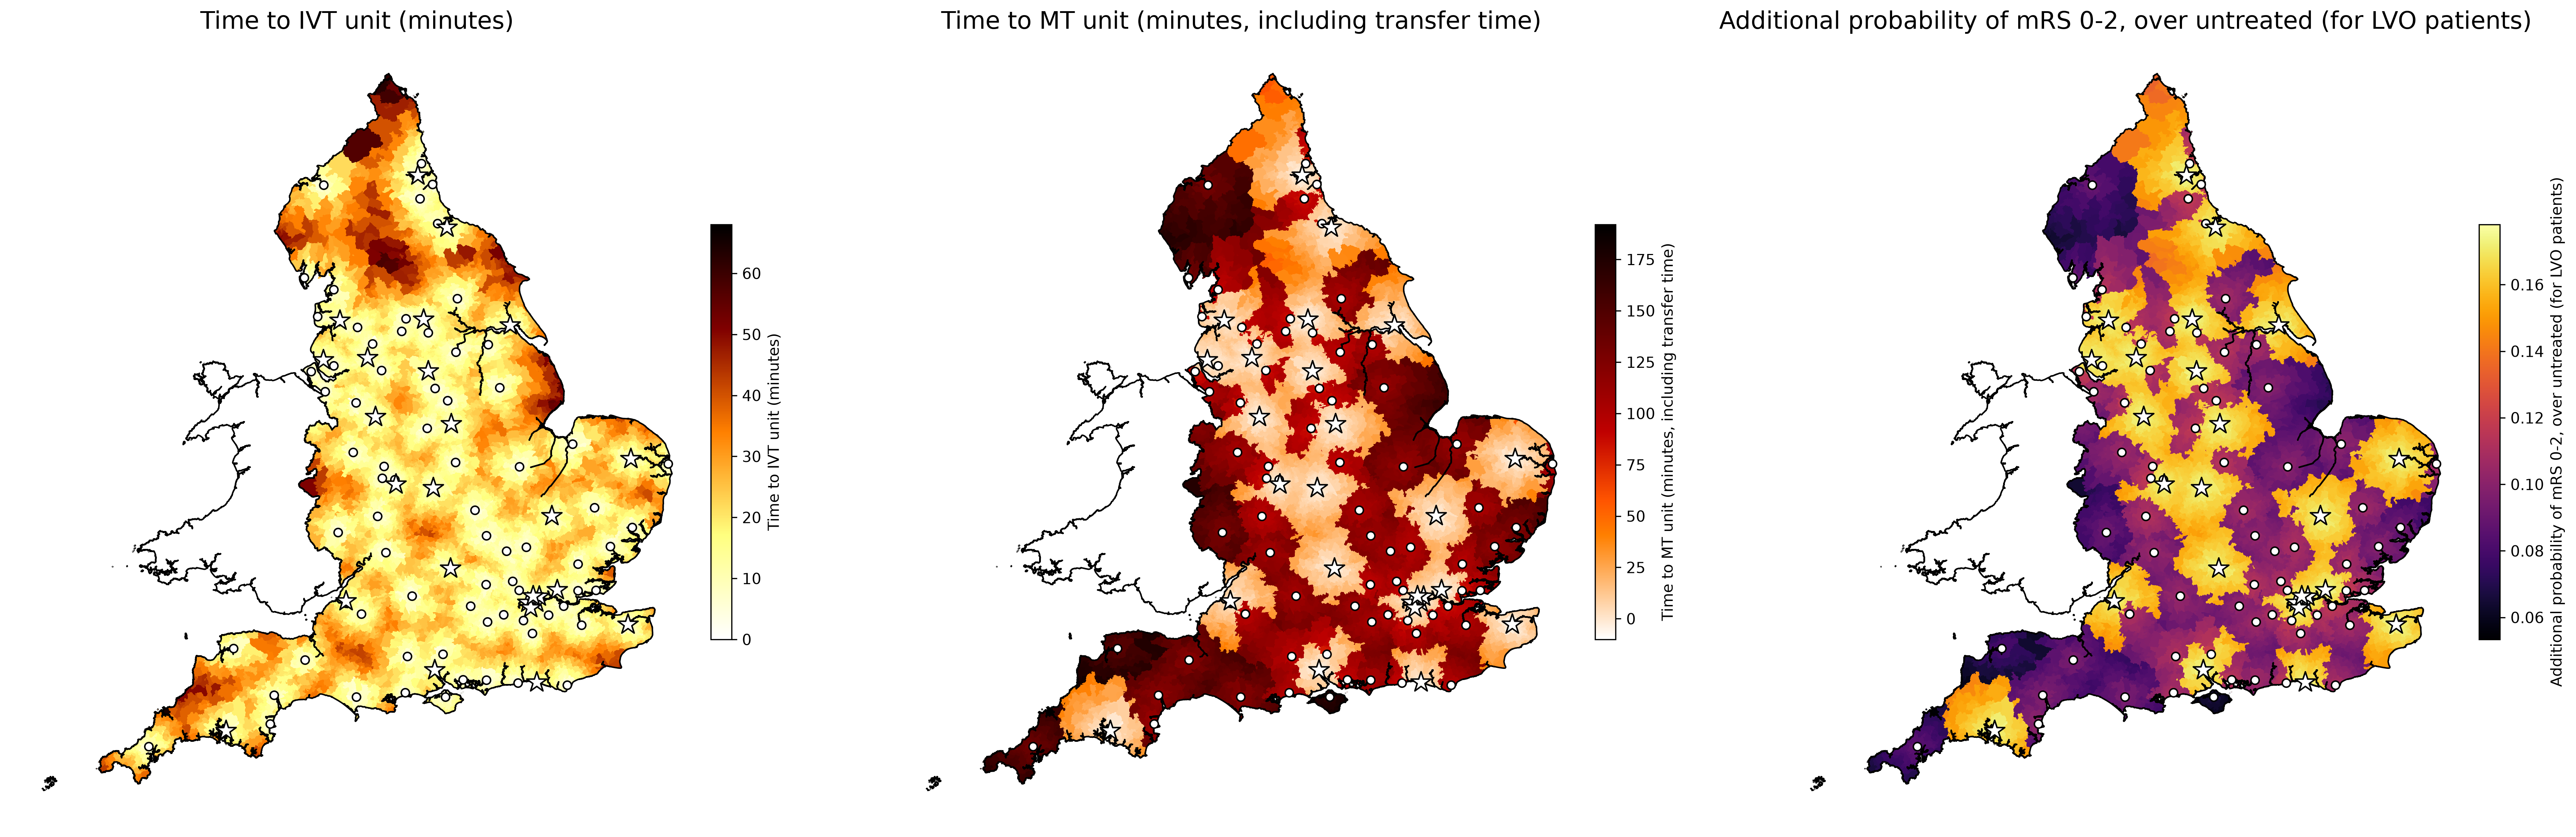
\includegraphics[width=1\linewidth]{images/map_three_in_one_current_hospitals_10min_travel_bias_lvo.png}
    \caption{Modelled times and outcomes for stroke patients with large vessel occlusion receiving thrombolysis (IVT) and thrombectomy (MT), with current IVT/MT provision (Taunton and Worcester as IVT-only units), no loss of MT by first attending an IVT-only unit, and with patients being taken to an MT unit if travel time is no longer than 10 minutes more than first attending a closer IVT-only unit. \textit{Left}: Predicted travel times to closest (in time) IVT unit. \textit{Middle}: Total travel time to MT unit; this includes travel time to closest IVT unit, a net delay before transfer of 60 minutes, and travel time from IVT unit to MT unit. \textit{Right}: The predicted improvement in the proportion of treated LVO patients with mRS 0-2 at 3-6 months, assuming there is no loss of use of MT by first attending an IVT-only unit. Stroke teams are shown as stars (providing both IVT and MT) or circles (providing IVT alone).}
    \label{fig:map_current_bias}
\end{figure}

\begin{figure}[H]
    \centering
    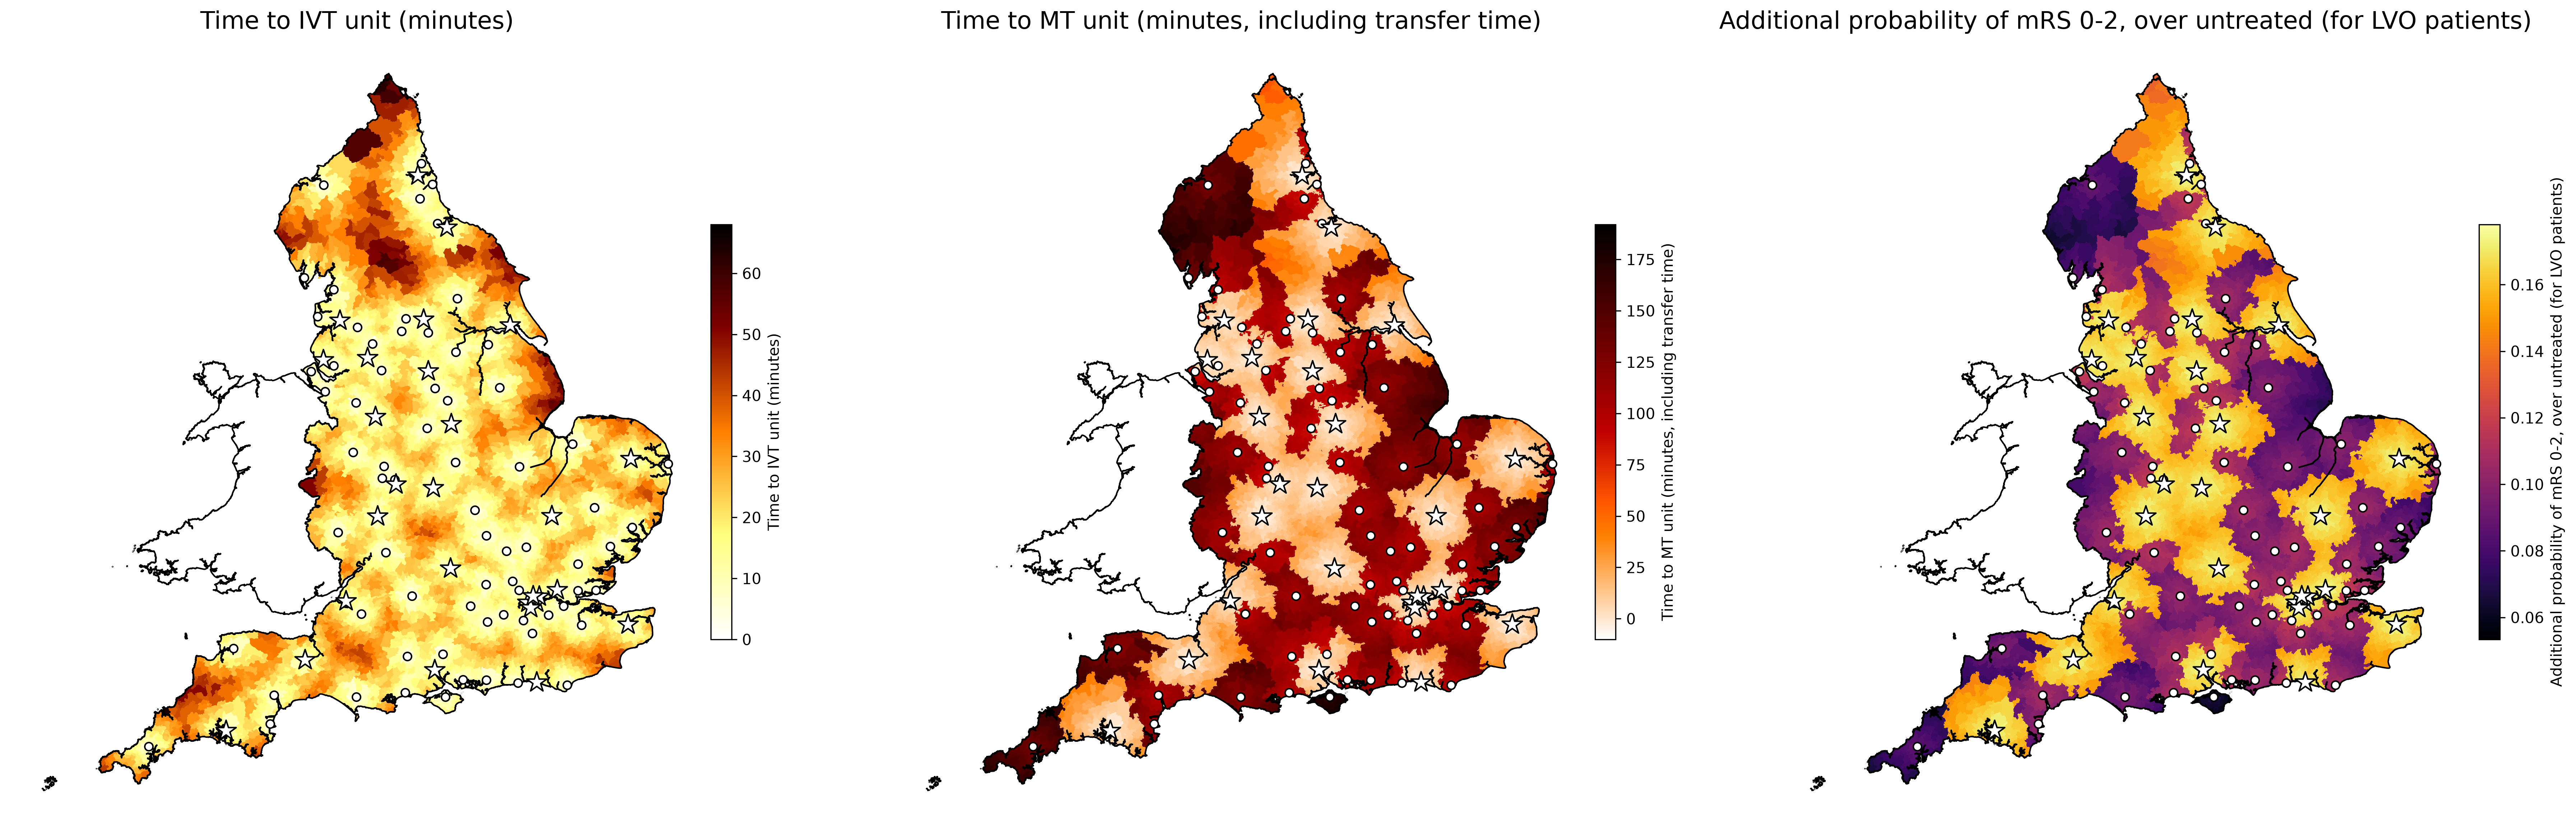
\includegraphics[width=1\linewidth]{images/map_three_in_one_taunton_and_worcester_10min_bias_lvo.png}
    \caption{Modelled times and outcomes for stroke patients with large vessel occlusion receiving thrombolysis (IVT) and thrombectomy (MT), with the addition of Taunton and Worcester providing MT, no loss of MT by first attending an IVT-only unit, and with patients being taken to an MT unit if travel time is no longer than 10 minutes more than first attending a closer IVT-only unit. \textit{Left}: Predicted travel times to closest (in time) IVT unit. \textit{Middle}: Total travel time to MT unit; this includes travel time to closest IVT unit, a net delay before transfer of 60 minutes, and travel time from IVT unit to MT unit. \textit{Right}: The predicted improvement in the proportion of treated LVO patients with mRS 0-2 at 3-6 months, assuming there is no loss of use of MT by first attending an IVT-only unit. Stroke teams are shown as stars (providing both IVT and MT) or circles (providing IVT alone).}
    \label{fig:map_taunton_worcester_bias}
\end{figure}
\section{Discussion}

\begin{itemize}
    \item Providing more thrombectomy centres improves outcomes, especially when placed in current ‘holes’ of good access to thrombectomy.
    \item The benefit is largest for the population naturally served by the new thrombectomy centre; benefit is less for transferred-in patients.
    \item If a patient first attends an IVT-only unit, they currently have a lower chance of receiving thrombectomy and, if they are transferred for thrombectomy, that thrombectomy will be be significantly delayed compared to first attending an MT-capable unit.
\end{itemize}

\bibliographystyle{naturemag}
%\bibliographystyle{plainnat}
%\bibliographystyle{unsrt}
%\bibliographystyle{unsrtnat}
\bibliography{references}

\subsection{Additional material}

\subsubsection{Disclaimer}

This report is independent research funded by the National Institute for Health and Care Research Applied Research Collaboration South West. The views expressed in this publication are those of the authors and not necessarily those of the National Institute for Health and Care Research or the Department of Health and Social Care.

\subsubsection{Geographic modelling disclaimer}

Geographic modelling is not an exact science applicable to every patient. It shows overall trends. Travel times each day, and in each location, may vary.

\begin{quote}
\textit{`I think you’re forgetting, Colin, that it’s half-term in North Wiltshire and West Somerset this week. It’ll be murder between Swindon and Warminster' ... `And there’s the Great West Steam Rally at Little Dribbling this weekend' somebody from across the room will add, strolling over to join you because it’s always pleasant to bring bad motoring news. `There’ll be 375,000 cars all converging on the Little Chef roundabout at Upton Dupton. We once spent eleven days in a tailback there, and that was just to get out of the car park'.} (Bill Bryson, Notes From A Small Island.)
\end{quote} 



\clearpage
\setcounter{section}{0}
\renewcommand{\thesection}{S\arabic{section}}
\section{Supplementary material}

\subsection{Selection of potential new MT units by net benefit}

\noindent
\begin{minipage}{\linewidth}
\centering
\captionof{table}{Order of benefit of adding a single new MT unit. Net benefit is a product of the overall catchment area for the new proposed MT unit (including the catchments of the IVT feeder units) and the benefit to those transferred to the new MT unit. \textit{Mean benefit for those benefiting} is the predicted improvement in percentage points of treated LVO patients with mRS 0-2 at 3-6 months, assuming there is no loss of use of MT by first attending an IVT-only unit.} 
\label{tab:hospital-benefit}
\begin{tabular}{r l r r r}
\toprule
Rank & Hospital Location & \shortstack{Admission Catchment\\Benefiting} & \shortstack{Mean Benefit for\\Those Benefiting} & \shortstack{Relative\\Net Benefit} \\
\midrule
1  & Harrow              & 6164 & 0.74 & 1.000 \\
2  & \textbf{Taunton}    & 2736 & 1.65 & 0.983 \\
3  & Exeter              & 2680 & 1.67 & 0.976 \\
4  & Watford             & 4980 & 0.87 & 0.944 \\
5  & Luton and Dunstable & 4456 & 0.96 & 0.930 \\
6  & Frimley Park        & 2705 & 1.53 & 0.904 \\
7  & Northampton         & 3458 & 1.17 & 0.884 \\
8  & Milton Keynes       & 2420 & 1.57 & 0.829 \\
9  & Chertsey            & 3320 & 1.09 & 0.785 \\
10 & Colchester          & 1332 & 2.70 & 0.784 \\
11 & Reading             & 4245 & 0.84 & 0.776 \\
12 & Bournemouth         & 2090 & 1.68 & 0.765 \\
13 & Truro               & 834  & 4.14 & 0.753 \\
14 & Peterborough        & 1716 & 1.93 & 0.722 \\
15 & Ipswich             & 1700 & 1.95 & 0.721 \\
16 & Torbay              & 2682 & 1.14 & 0.666 \\
17 & Stevenage           & 3367 & 0.84 & 0.620 \\
18 & Dartford            & 2879 & 0.98 & 0.615 \\
19 & Wolverhampton       & 3279 & 0.86 & 0.615 \\
20 & High Wycombe        & 5329 & 0.52 & 0.605 \\
21 & Cheltenham          & 2762 & 1.00 & 0.604 \\
22 & \textbf{Worcester}  & 2010 & 1.37 & 0.600 \\
23 & Carlisle            & 683  & 4.02 & 0.597 \\
24 & Lincoln             & 917  & 2.99 & 0.597 \\
25 & Portsmouth          & 1980 & 1.37 & 0.592 \\
\bottomrule
\end{tabular}
\end{minipage}

\end{document}